\documentclass{article}
\usepackage{graphicx}
\usepackage{float}

\usepackage{booktabs}
\usepackage{tabularx}
\usepackage{hyperref}
\usepackage{pdflscape}
\usepackage{ltablex}
\usepackage{lipsum}

\keepXColumns

% Defines new column types that use ragged right so the table doesn't look awful
\newcolumntype{Y}{>{\raggedright\arraybackslash}X}
\newcolumntype{P}[1]{>{\raggedright\arraybackslash}p{#1}}

\hypersetup{
    colorlinks=true,       % false: boxed links; true: colored links
    linkcolor=red,          % color of internal links (change box color with linkbordercolor)
    citecolor=green,        % color of links to bibliography
    filecolor=magenta,      % color of file links
    urlcolor=cyan           % color of external links
}

\title{Hazard Analysis\\\progname}

\author{\authname}

\date{}

%% Comments

\usepackage{color}

\newif\ifcomments\commentstrue %displays comments
%\newif\ifcomments\commentsfalse %so that comments do not display

\ifcomments
\newcommand{\authornote}[3]{\textcolor{#1}{[#3 ---#2]}}
\newcommand{\todo}[1]{\textcolor{red}{[TODO: #1]}}
\else
\newcommand{\authornote}[3]{}
\newcommand{\todo}[1]{}
\fi

\newcommand{\wss}[1]{\authornote{magenta}{SS}{#1}} 
\newcommand{\plt}[1]{\authornote{cyan}{TPLT}{#1}} %For explanation of the template
\newcommand{\an}[1]{\authornote{cyan}{Author}{#1}}

%% Common Parts

\newcommand{\progname}{Software Engineering} % PUT YOUR PROGRAM NAME HERE
\newcommand{\authname}{Team 8, RLCatan
\\ Rebecca Di Filippo
\\ Jake Read
\\ Matthew Cheung
\\ Sunny Yao} % AUTHOR NAMES

\usepackage{hyperref}
    \hypersetup{colorlinks=true, linkcolor=blue, citecolor=blue, filecolor=blue,
                urlcolor=blue, unicode=false}
    \urlstyle{same}
                                


\begin{document}

\maketitle
\thispagestyle{empty}

~\newpage

\pagenumbering{roman}

\begin{table}[hp]
\caption{Revision History} \label{TblRevisionHistory}
\begin{tabularx}{\textwidth}{llX}
\toprule
\textbf{Date} & \textbf{Developer(s)} & \textbf{Change}\\
\midrule
Date1 & Name(s) & Description of changes\\
Date2 & Name(s) & Description of changes\\
... & ... & ...\\
\bottomrule
\end{tabularx}
\end{table}

~\newpage

\tableofcontents

~\newpage

\pagenumbering{arabic}

\wss{You are free to modify this template.}

\section{Introduction}

\wss{You can include your definition of what a hazard is here.}

A hazard is defined as a property or condition in the system together
with a condition in the environment that has the potential to cause harm or
damage. We define harm as the underperformance of our system
that leads to the incorrect instruction of players. In addition, we consider
disruption of play, loss of game data/state as harm.


\section{Scope and Purpose of Hazard Analysis}

\wss{You should say what \textbf{loss} could be incurred because of the
hazards.}


The loss that can be incurred because of the hazards include the
forfeiture or inability to continue a game of Catan. This can affect the
user experience of our software and lead to a loss of trust in the product.


\section{System Boundaries and Components}

\wss{Dividing the system into components will help you brainstorm the hazards.
You shouldn't do a full design of the components, just get a feel for the major
ones.  For projects that involve hardware, the components will typically include
each individual piece of hardware.  If your software will have a database, or an
important library, these are also potential components.}



Components: 
\begin{itemize}

\item User Interface
\item Game State Digital Twin
\item AI Model
\item Board Representation
\item Game State Database
\item Camera Feed

\end{itemize}

\begin{figure}[H]
    \centering
    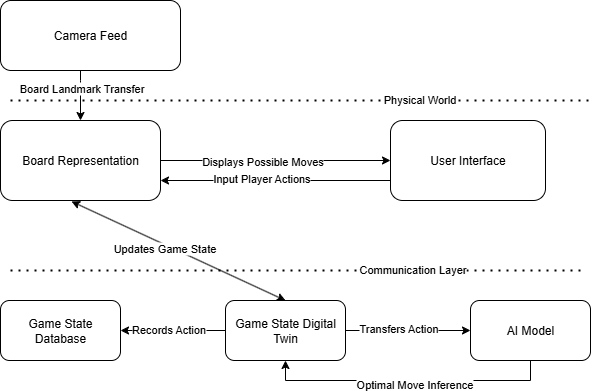
\includegraphics[width=\textwidth]{Component_Diagram_hazards.png}
    \caption{\textit{System components: User Interface, Game State Digital Twin, AI Model, Board Representation, Game State Database, and Camera Feed.}}
    \label{fig:component-diagram}
\end{figure}

\section{Critical Assumptions}

\wss{These assumptions that are made about the software or system.  You should
minimize the number of assumptions that remove potential hazards.  For instance,
you could assume a part will never fail, but it is generally better to include
this potential failure mode.}


We assume that the users of our system will be familiar with the rules of Catan and
know how to play the game. Another assumption is that the users will have a basic understanding
of how to interact with a digital interface. Finally, we assume that existing consumer
hardware will be able to run full-depth processing of our AI model.

\section{Failure Mode and Effect Analysis}

\wss{Include your FMEA table here. This is the most important part of this document.}
\wss{The safety requirements in the table do not have to have the prefix SR.
The most important thing is to show traceability to your SRS. You might trace to
requirements you have already written, or you might need to add new
requirements.}
\wss{If no safety requirement can be devised, other mitigation strategies can be
entered in the table, including strategies involving providing additional
documentation, and/or test cases.}

% Finally, a table that spans multiple pages and doesn't look horrendous, only took 2 hours to get the formatting right...
\begin{landscape}
    % Layout setup
    \renewcommand{\arraystretch}{1.3}
    \begin{tabularx}{\linewidth}{|P{2.5cm}|Y|Y|Y|Y|P{1cm}|P{1cm}|}

        % Header
        \caption{Failure Mode and Effect Analysis (FMEA)} \\
        \hline
        \textbf{Design Function} &
        \textbf{Failure Modes} &
        \textbf{Effects of Failure} &
        \textbf{Causes of Failure} &
        \textbf{Recommended Action} &
        \textbf{SR} &
        \textbf{Ref.} \\
        \hline
        \endfirsthead

        % Subsequent pages header
        \hline
        \textbf{Design Function} &
        \textbf{Failure Modes} &
        \textbf{Effects of Failure} &
        \textbf{Causes of Failure} &
        \textbf{Recommended Action} &
        \textbf{SR} &
        \textbf{Ref.} \\
        \hline
        \endhead

        % Prompt that the table continues
        \hline
        \multicolumn{7}{r}{\textit{Continued on next page}} \\
        \endfoot

        % No footer on last page
        \hline
        \endlastfoot

        % Table Rows...

        \raggedright
        Board Representation &
        Incorrect parsing of the physical board state (e.g., misidentifies road or settlement). &
        AI advice is based on false information, leading to invalid or poor recommendations. &
        CV model misclassifies pieces due to lighting, angle, or occlusion. &
        Give the option for users to manually confirm the parsed board state before generating advice. &
        SR-1 &
        H1-a \\

        \hline

        Game State Digital Twin &
        Loss of synchronization between physical game and digital twin. &
        System provides advice for the wrong game state, disrupting play. &
        Failure to read new game state to model, or additional moves made by players after CV scan. &
        Provide a resynchronization mechanism, such as an option to rescan the board or manually enter current state. &
        SR-2 &
        H2-a \\

        \hline

        AI Model &
        AI suggests an illegal or nonsensical move. &
        Users may become confused or game flow disrupted if they attempt an invalid action. &
        AI loses track of game state or misinterprets or rules are not properly encoded. &
        AI-suggested moves are validated against the official rules of Catan before display. &
        SR-3 &
        H3-a \\

        \hline

        User Interface &
        Advice not displayed on time. &
        Player's turn timer runs out, causing them to miss their turn as they wait. &
        Model takes too long to compute next move, or there are delays in CV processing. &
        Limit the processing time of the model or timeout early and inform user of failure before their turn ends. &
        SR-4 \newline SR-5 &
        H4-a \\

        \hline

        Game State Database &
        Failure to save game states. &
        LLM is unable to summarize "what could have been" from previous game states. &
        Game moves too quickly for state to be saved (Mostly applicable to bot vs. bot games). &
        Ensure that the current game state is saved correctly before the recommended move is sent to the user. &
        SR-6 &
        H5-a \\

        \hline

        Communication Layer (Phone/Server) &
        Dropped connection between user device and processing server. &
        Advice delayed or not delivered, leading to disrupted play. &
        External server goes down, or WiFi connectivity issues occur. &
        Attempt to reconnect, and notify the user that connection has dropped. &
        SR-7 \newline SR-8 &
        H6-a \\

        \hline

        Visualization &
        Incorrect or confusing rendering of the game state. &
        Players misinterpret advice or system status, leading to wrong actions. &
        Suggested move is not easy to quickly spot on the displayed board. &
        Visually distinguish the move(s) suggested by AI, e.g., using highlights or arrows. &
        SR-9 &
        H7-a \\

    \end{tabularx}
\end{landscape}

\section{Safety and Security Requirements}

\wss{Newly discovered requirements.  These should also be added to the SRS.  (A
rationale design process how and why to fake it.)}

The following safety and security requirements have been derived from the hazard analysis above.
Each requirement is traced to a hazard in the FMEA table (Table 3):

\begin{itemize}
    \item SR-1: The system shall enable users to manually confirm the parsed board state before generating advice.
    \item SR-2: The system shall provide a resynchronization mechanism (manual correction or re-scan).
    \item SR-3: The system shall validate all AI-suggested moves against the official rules of Catan before display.
    \item SR-4: The system shall ensure advice is displayed within 5 seconds of request.
    \item SR-5: The system shall provide a clear error message if advice cannot be generated.
    \item SR-6: The system shall ensure current game state is saved correctly before recommending move(s) to the user.
    \item SR-7: The system shall notify the user of connection loss within 5 seconds.
    \item SR-8: The system shall attempt automatic reconnection at least 3 times before failing.
    \item SR-9: The system shall visually distinguish the move(s) suggested by AI.
\end{itemize}


\section{Roadmap}

\wss{Which safety requirements will be implemented as part of the capstone timeline?
Which requirements will be implemented in the future?}

The following requirements will be implemented as part of the capstone timeline:
\begin{itemize}
    \item SR-1: Being able to confirm the board state is crucial in the early stages to ensure the system is functioning correctly.
          It will be valuable for both users and developers to have this feature implemented early.
    \item SR-2: Resynchronization is important to maintain the integrity of the game state.
          This feature will help recover from potential errors in board state detection, which is likely to occur during initial testing and development.
    \item SR-3: If the AI suggests illegal moves, the entire purpose of the system is defeated.
          This requirement is essential to ensure the system provides valid advice.
    \item SR-5: Clear error messages are important not only for user experience but also for debugging during development, so it makes sense to add them early.
    \item SR-6: The issues caused by game states not being saved correctly will likely be a problem primarily in bot vs. bot games.
          This will be most useful while training the AI, which is naturally within the scope of the capstone.
    \item SR-9: Clear visualization of AI suggestions is important for user experience and should be relatively straightforward to implement.
          This will help users quickly understand the AI's advice, which is a core functionality of the system.
\end{itemize}

The following requirements are planned for future implementation:
\begin{itemize}
    \item SR-4: While timely advice is important, it may be challenging to guarantee a strict time limit during the initial development phase.
    \item SR-7: Connection loss handling is important, but it may be less critical during initial development when the focus is on core functionalities.
          For now we'll assume a stable connection.
    \item SR-8: See SR-7.
\end{itemize}


\newpage{}

\section*{Appendix --- Reflection}

\wss{Not required for CAS 741}

% The purpose of reflection questions is to give you a chance to assess your own
learning and that of your group as a whole, and to find ways to improve in the
future. Reflection is an important part of the learning process.  Reflection is
also an essential component of a successful software development process.  

Reflections are most interesting and useful when they're honest, even if the
stories they tell are imperfect. You will be marked based on your depth of
thought and analysis, and not based on the content of the reflections
themselves. Thus, for full marks we encourage you to answer openly and honestly
and to avoid simply writing ``what you think the evaluator wants to hear.''

Please answer the following questions.  Some questions can be answered on the
team level, but where appropriate, each team member should write their own
response:


\begin{enumerate}
    \item What went well while writing this deliverable? 
    \item What pain points did you experience during this deliverable, and how
    did you resolve them?
    \item Which of your listed risks had your team thought of before this
    deliverable, and which did you think of while doing this deliverable? For
    the latter ones (ones you thought of while doing the Hazard Analysis), how
    did they come about?
    \item Other than the risk of physical harm (some projects may not have any
    appreciable risks of this form), list at least 2 other types of risk in
    software products. Why are they important to consider?
\end{enumerate}

\subsection*{Jake Read}\label{subsec:jake-read-reflection}
\begin{enumerate}
    \item For the most part, this delivery went rather smoothly.
    Our project was rather simple to separate into components and boundaries, which made getting started quite simple.
    Once everything was set up, it wasn't too hard to think up potential hazards, and the requirements stemming from them quickly became clear.
    Overall I had a much more enjoyable time working on this deliverable than I did on the SRS.

    \item Funnily enough, the most challenging part of this deliverable for me was setting up the FMEA table.
    Getting the formatting right took a lot of trial and error, and I had to look up a lot of documentation to figure out how to get the table to look decent.
    It's just so wide, and has to span multiple pages, which made it difficult to get right.
    It took about as long to format the table as it did to fill it in the end.

    \item We hadn't really considered much in regard to risk before this document.
    That being said, there are some risks that were pretty obvious given the nature of the project, such as the CV component misreading the board state.
    Ones like this we had in the back of our minds, so they were quick to put into words.
    Other risks, such as loss of synchronization between the physical and digital board, were things we hadn't really thought of before.
    The idea occurred to me while trying to think of potential failure modes for the digital twin component, so I reached out to our supervising professor to see if it was a valid concern.
    He agreed that it was, so I added it to the table.
    Another category of risks we hadn't considered were the ones related to connectivity issues.
    (Well, maybe the rest of the team had thought of them, but it hadn't crossed my mind.)
    These came directly from thinking about what could go wrong with the communication layer component, so it's cool to see how the hazard analysis process can actually lead to new insights.
    To be honest, I'm typically fairly skeptical of how helpful a lot of documentation-heavy deliverables are, but this one I can actually see the value in.

    \item As I mentioned above, one of the major sources of risk in software products is connectivity issues.
    It's easy to forget that not all users will have a perfect internet connection, and that servers can go down, when you're in the middle of development.
    If you don't have a plan when you do run into these issues, it can be a bit of a pain to deal with.
    Obviously another type of risk is security vulnerabilities.
    It's not really relevant to our project since we don't handle sensitive data, which is why we don't have hazards relating to it.
    For software that does handle sensitive data, it's of course not something you can just ignore.
    User data getting leaked is a big issue that will negatively impact the users and could potentially lead to legal troubles.
\end{enumerate}

\end{document}